\chapter{Hardware und Software}
Dieses Kapitel führt die gegebenen und verwendeten Hard- und Software Komponenten in dieser Arbeit auf.

\section{Der Kaffeevollautomat}
Der "`Jura Impressa S9"', siehe Abbildung \ref{subfig:Kaffeevollautomat}, ist ein Kaffeevollautomat mit fünf Kaffeebezugstasten: Spezialkaffee, 1 große Tasse Kaffee, 2 große Tassen Kaffee, 1 kleine Tasse Kaffee und 2 kleine Tassen Kaffee.
Auf der rechten Seite befinden sich Bedienelemente für heißes (Tee-)Wasser und Wasserdampf zum Milch Aufschäumen.
Der Kaffeevollautomat wird für seinen Betrieb direkt mit der Netzspannung versorgt.

% \begin{figure}
%   \begin{center}
%     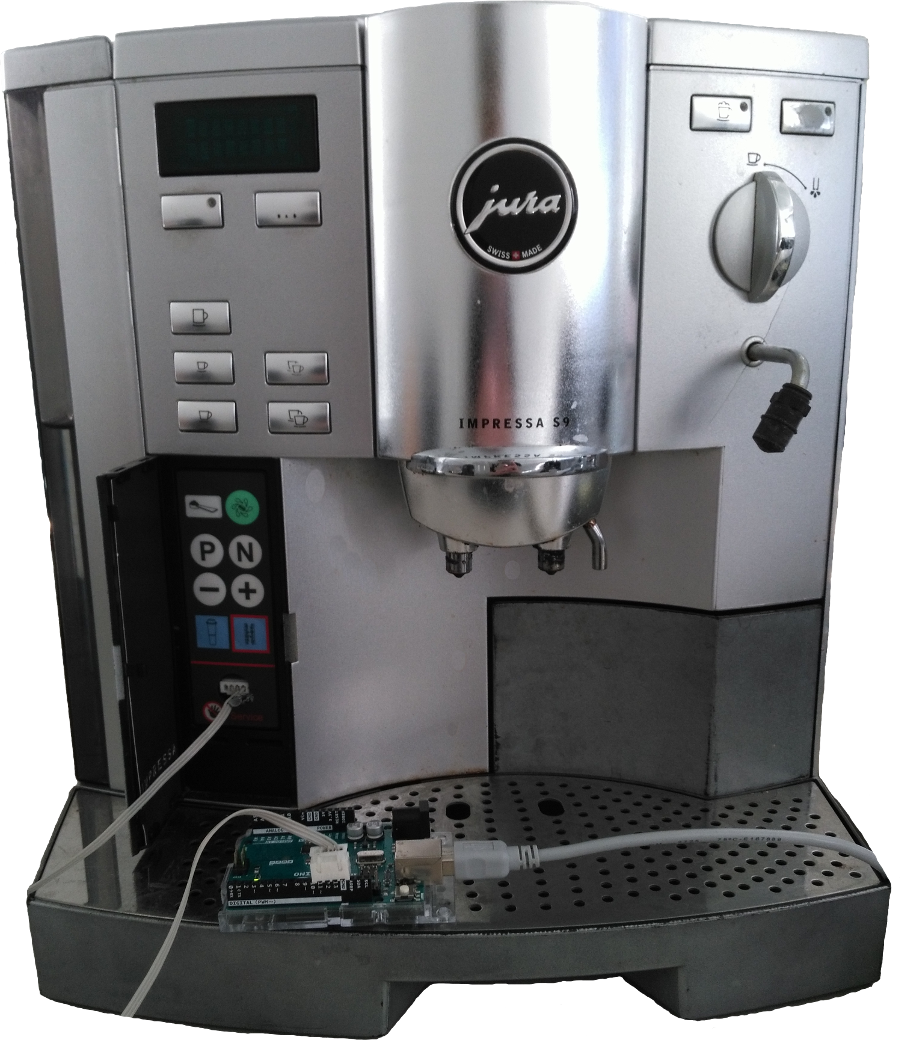
\includegraphics[scale=0.2]{images/Jura-Impressa-S9-small}
%     \caption{Jura Impressa S9 -- Kaffeevollautomat}
%     \label{fig:Kaffeevollautomat}
%   \end{center}
% \end{figure}

% \begin{figure}
%   \begin{subfigure}{.45\textwidth}
%     \centering
%     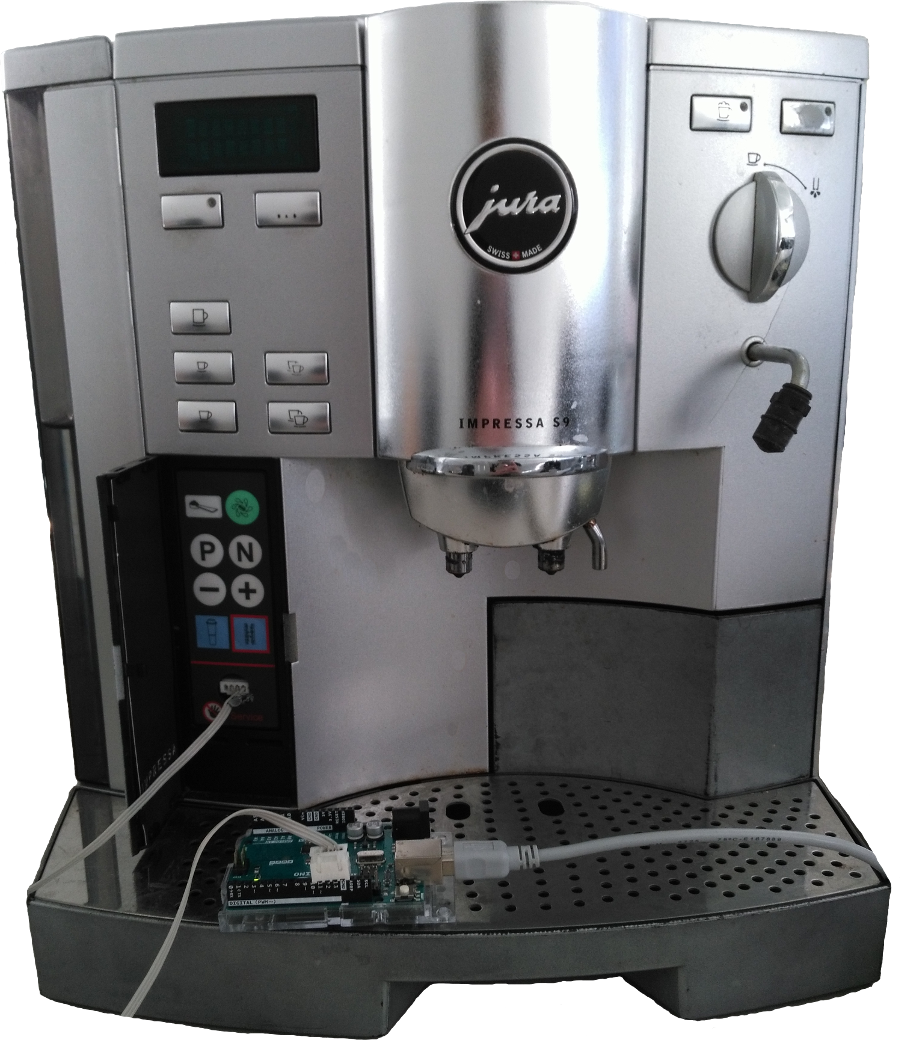
\includegraphics[scale=0.2]{images/Jura-Impressa-S9-small}
%     \caption{Jura Impressa S9 -- Kaffeevollautomat}
%     \label{fig:Kaffeevollautomat-xxxxxxxxxxxxxxxxxxxxxxxxxxxxxxxxxxxxxxxxxxxxxxxxxxxxxxxxxxxxxxxxxxxxxxxxxxxxxxxxxxxxxxxxxxx}
%   \end{subfigure}
%   \hfill
%   \begin{subfigure}{.45\textwidth}
%     \centering
%     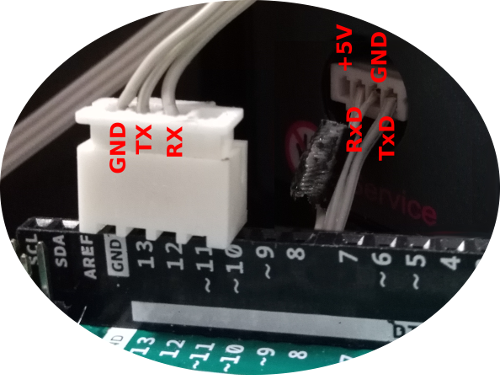
\includegraphics[scale=0.3]{images/Jura-Arduino-Pins-beschriftet-small}
%     \caption{Pinbelegung: Jura Impressa S9 -- Arduino Uno}
%     \label{fig:KaffeevollautomatPins-xxxxxxxxxxxxxxxxxxxxxxxxxxxxxxxxxxxxxxxxxxxxxxxxxxxxxxxxxxxxxxxxxxxxxxxxxxxxxxxxxxxxxx}
%   \end{subfigure}
% \end{figure}

\subfigbox{
  \subfigure[Der ganze Kaffeevollautomat]{\label{subfig:Kaffeevollautomat}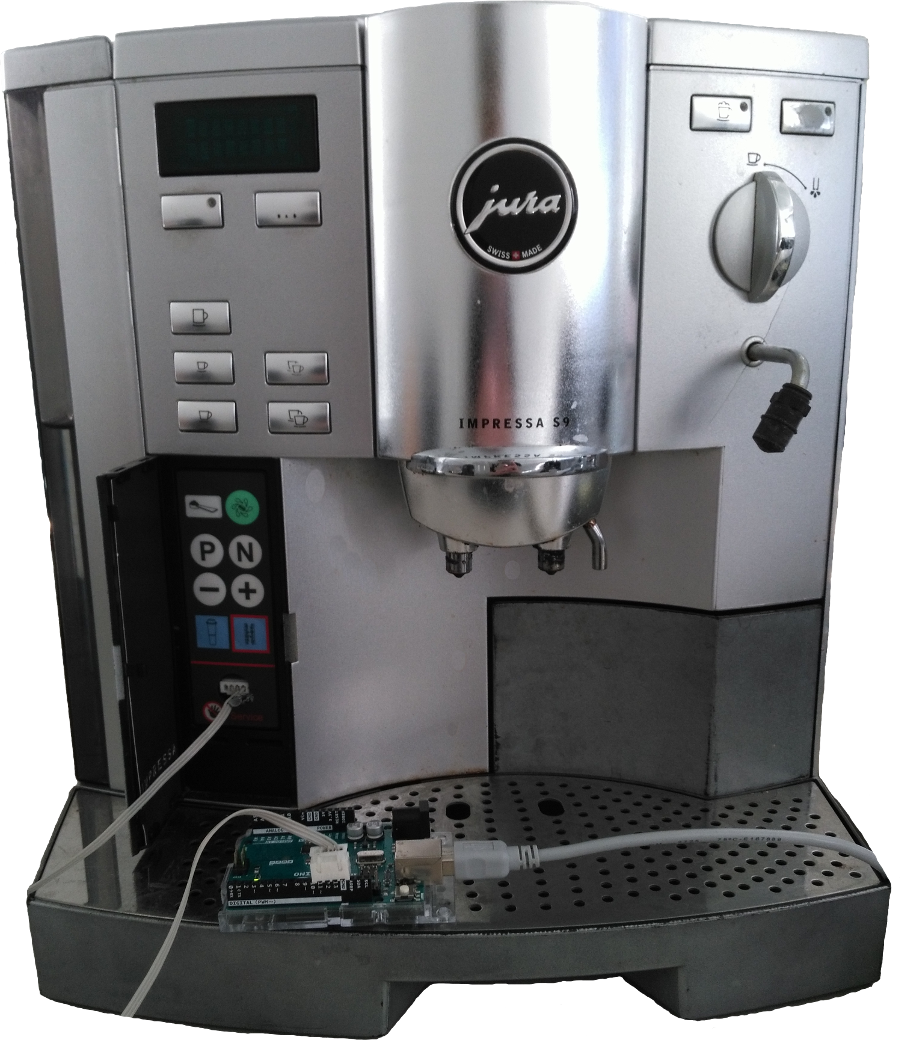
\includegraphics[scale=0.2]{images/Jura-Impressa-S9-small}}\hfill%
  \subfigure[Pinbelegung zum Arduino Uno]{\label{subfig:KaffeevollautomatPins}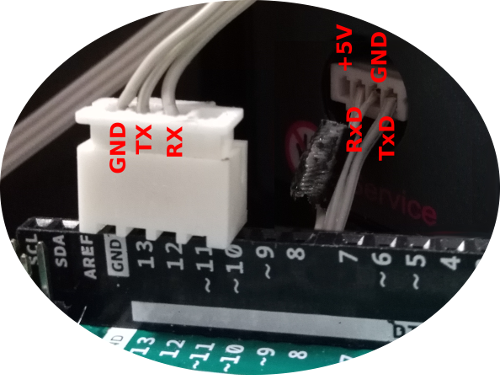
\includegraphics[scale=0.3]{images/Jura-Arduino-Pins-beschriftet-small}}%
}{Jura Impressa S9}{fig:Kaffeevollautomat}

\subsection{Aufbau und Verkabelung}
Hinter der linken Wartungsklappe an der Vorderseite des Kaffeevollautomaten befindet sich neben mehreren Menü-Tasten auch eine serielle Schnittstelle.
Über ein eigenes \ac{UART} Protokoll kann hierüber mit der Maschine kommuniziert werden.

Abbildung \ref{subfig:KaffeevollautomatPins} illustriert die Pinbelegung.
Die 5 Volt Leitung kann für ein autark laufendes Projekt genutzt werden.
In dieser Arbeit bezieht der Arduino seine Versorgungsspannung über den am USB Kabel befindlichen Computer.
Von \texttt{TX} nach \texttt{RxD} werden Befehle an den Kaffeevollautomaten verschickt.
Auf der Rückrichtung von \texttt{TxD} nach \texttt{RX} werden Antworten des Kaffeevollautomaten gelesen.
\texttt{GND} ist abschließend die gemeinsame Erdung und Bezugsleitung für die serielle Kommunikation.
Auf der Abbildung kreuzen sich die Leitungen \texttt{RxD} und \texttt{GND} am Stecker auf Seiten des Kaffeevollautomaten.
\texttt{GND} ist über eine schwarze Markierung gekennzeichnet.

Ein Arduino Uno übersetzt als "`Man in the middle"' die bekannten Kommandos in das Format der Kaffeemaschine.
Sie serielle Kommunikation läuft über die Pins Nummer 12 und 13.
Über eine weitere serielle Verbindung per USB lässt sich der Arduino ansteuern.

Aus Sicht des Computers ist der Arduino ein Gerätelaufwerk unter \texttt{/dev/ttyACM0} mit einer Baudrate von 9600.
Diese Zahl findet sich zu Beginn des Arduino Uno Skripts aus dem Projekt "`CoffeeMachine"'\cite{GitCoffeeMachine} wieder.

% \begin{figure}
%   \begin{center}
%     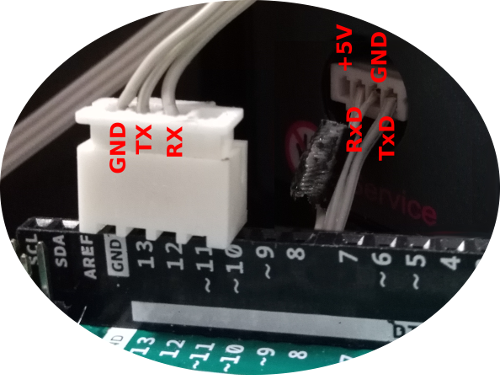
\includegraphics[scale=0.3]{images/Jura-Arduino-Pins-beschriftet-small}
%     \caption{Pinbelegung: Jura Impressa S9 -- Arduino Uno}
%     \label{fig:KaffeevollautomatPins}
%   \end{center}
% \end{figure}

\subsection{Kommandos}\label{subsec:Kommandos}
Die Tabelle~\ref{tbl:kommandos} zeigt die Befehlsgruppen, sowie ausgewählte Befehle, die der Kaffeevollautomat versteht.
Diese Befehle stammen aus dem Git Repository \cite{GitCoffeeMachine}, worauf diese Arbeit aufbaut.

Befehle beginnen entweder mit zwei Großbuchstaben gefolgt von einem Doppelpunkt und i.d.R. einer zweistelligen Hexadezimalzahl, oder sie beginnen mit einem Fragezeichen gefolgt von i.d.R. zwei ASCII Zeichen.
Positionsnummern, egal ob Speicherposition, \mbox{Betriebszustands-,} Bezugstasten- oder Steuerungskomponenten-Nummer, werden durch zweistellige Hexadezimalzahlen repräsentiert und reichen von $0_{16}=0_{10}$ bis FF$_{16}=255_{10}$.

Zwei Ausnahmen des ersten Typs sind z.B. \texttt{TY:} zum Abfragen des Maschinen Typs und \texttt{WE:00,01FF} zum Schreiben des Wertes $01$FF$_{16} = 511_{10}$ an die Position $00$.
Eine Ausnahme des zweiten Typs ist z.B. \texttt{?D1DISPLAY}\textvisiblespace\ und \texttt{?D2}\textvisiblespace\textvisiblespace\texttt{TEST}\textvisiblespace\textvisiblespace.
Der volle Umfang möglicher Displayzeichen, sowie deren Benutzung wird in Abschnitt \ref{sec:Display} ausgeführt.

Einige Befehle, die aus weiteren Projekten mit Maschinen der S-Reihe bekannt sind, sind in dieser "`Jura Impressa S9"' leider nicht implementiert.
Dazu zählen \texttt{IC:} zum Auslesen aller Eingaben, \texttt{FA:0A} eine unbelegte Bezugstaste, \texttt{CM:} für weitere Status Informationen, \texttt{CS:} für Sensor Informationen und \texttt{PM:} ein Befehl um Musik abzuspielen.
Weitere Befehlsgruppen werden in der \texttt{README.rst} eines Github Repositories aufgeführt\footnote{\url{https://github.com/PromyLOPh/juramote}}.

\begin{tuhhtable}
  \footnotesize\centering
  \begin{tabular}[tp]{L{.22\textwidth}L{.48\textwidth}L{.18\textwidth}}
%
  \THc{1}{c}{Kommando} & \THc{1}{c}{Beschreibung} & \THc{1}{c}{Rückgabewert} \\
%
  \TRx{3}{l}{Betriebszustand (AN:<id>)}\\
  \abovebodyrule
  AN:01    & Einschalten        & ok:    \\\TRc
  AN:02    & Ausschalten        & ok:    \\
  AN:03    & Display Test       & ok:    \\\TRc
  AN:<id>  & u.v.m.             & ok:    \\
  \belowbodyrule
%
  \TRx{3}{l}{Bezugstaste (FA:<id>)}\\
  \abovebodyrule
  FA:02    & Gerät spülen       & ok:    \\\TRc
  FA:0C    & Spezialkaffee      & ok:    \\
  FA:<id>  & u.v.m.             & ok:    \\\TRc
  \belowbodyrule
%
  \TRx{3}{l}{Steuerungskomponenten (FN:<id>)}\\
  \abovebodyrule
  FN:<id>  & Pumpen, Heizung, u.v.m & ok:    \\\TRc
  \belowbodyrule
%
  \TRx{3}{l}{Eingabestatus*}\\
  \abovebodyrule
  IC:      & Eingaben auslesen* &        \\\TRc
  \belowbodyrule
%
  \TRx{3}{l}{Spiele Musik (easter egg)*}\\
  \abovebodyrule
  PM:      & Play music*        &        \\\TRc
  \belowbodyrule
%
  \TRx{3}{l}{Speicherzugriff}\\
  \abovebodyrule
  RE:<address> & Liest 2 Byte EEPROM Speicher   & re:[0000-FFFF] \\\TRc
  WE:<address>,<value> & Schreibt 2 Byte in EEPROM & ok:         \\
  RT:<address> & Liest eine Zeile EEPROM        & rt:[0-F 64x]   \\\TRc
  RR:<address> & Liest eine Zeile RAM           & rr:[0-F 32x]   \\
  \belowbodyrule
%
  \TRx{3}{l}{Sperrung}\\
  \abovebodyrule
  ?M3      & Aktiviert den Inkassomodus         & ?ok            \\\TRc
  ?M1      & Deaktiviert den Inkassomodus       & ?ok            \\
  \belowbodyrule
%
  \TRx{3}{l}{Display}\\
  \abovebodyrule
  ?D0      & Standard Displaytext zurück setzen & ?ok            \\\TRc
  ?D1[A-Z 8-11x] & Displaytext Zeile 1          & ?ok            \\
  ?D2[A-Z 8-11x] & Displaytext Zeile 2          & ?ok            \\\TRc
  \belowbodyrule
%
  \TRx{3}{l}{Aktion an der Kaffeemaschine}\\
  \abovebodyrule
           & 1 kleiner Kaffee (Produkt 1)       & ?PAE         \\\TRc
           & 2 kleine Kaffees (Produkt 2)       & ?PAF         \\
           & 1 großer Kaffee  (Produkt 3)       & ?PAA         \\\TRc
           & 2 große Kaffees  (Produkt 4)       & ?PAB         \\
           & Spezialkaffe     (Produkt 7)       & ?PAG         \\\TRc
           & Dampf            (Produkt 6)       & ?PAI         \\
           & 1 Dampfportion   (Produkt 5)       & ?PAJ         \\\TRc
           & 1 Tasse Tee      (Produkt 8)       & ?PAK         \\
  \belowbodyrule
%
  \TRx{3}{l}{* leider nicht alles in der Jura Impressa S9 implementiert, siehe weitere Geräte der S-Reihe}\\
%
  \end{tabular}
  \caption{Befehlsübersicht der Jura Kaffeevollautomaten (S-Reihe)}
  \label{tbl:kommandos}
\end{tuhhtable}

\subsection{Serielle Kommunikation}
Das Arduino Skript aus dem Projekt "`CoffeeMachine"'\cite{GitCoffeeMachine} wird als Grundlage der Kommunikation in dieser Arbeit weiter verwendet.
Es kodiert die \ac{UART} Kommandos von und zu dem Kaffeevollautomaten.

Die Befehle aus der Kommando Tabelle~\ref{tbl:kommandos} werden zeichenweise ASCII-Zeichen für Zeichen übertragen.
Dafür wird ein an den Kaffeevollautomaten adressiertes Byte (ein ASCII-Zeichen), bestehend aus acht Bits, in je vier Bytes aufgeteilt.
Die dritte und sechste Stelle der neuen Bytes repräsentieren je zwei Bits des ursprünglichen Bytes.
Bei der Übertragung an den Kaffeevollautomaten werden die restlichen Bits mit Nullen aufgefüllt.
Abbildung \ref{fig:uart} veranschaulicht dies an dem ersten Byte des Einschaltbefehls, die entsprechende ASCII-Kodierung ist in Abbildung \ref{tbl:Displaysymbole} der zweiten und dritten Spalte zu entnehmen.
Die Kodierung der, von dem Kaffeevollautomaten kommenden, Bytes erfolgt analog.
Laut "`Protocoljura"'\footnote{\url{http://protocoljura.wiki-site.com/index.php/Protocol_to_coffeemaker}} bestehen die irrelevanten Bits der ankommenden Bytes aus einer Null und weiteren fünf Einsen pro Byte.

Vier Bytes kodieren auf diese Weise ein ASCII Zeichen und werden fortan als Gruppe bezeichnet.
Zwischen jeder Gruppe gibt es eine Verzögerung von 8ms.
Diese Verzögerung begrenzt hauptsächlich die Übertragungsgeschwindigkeit, was in Abschnitt \ref{subsec:zugangSeriellDirekt} diskutiert wird.

Die jetzt vorhandene Umgebung kann bereits über den seriellen Monitor der Arduino IDE genutzt werden.

\begin{figure}
  \begin{center}
    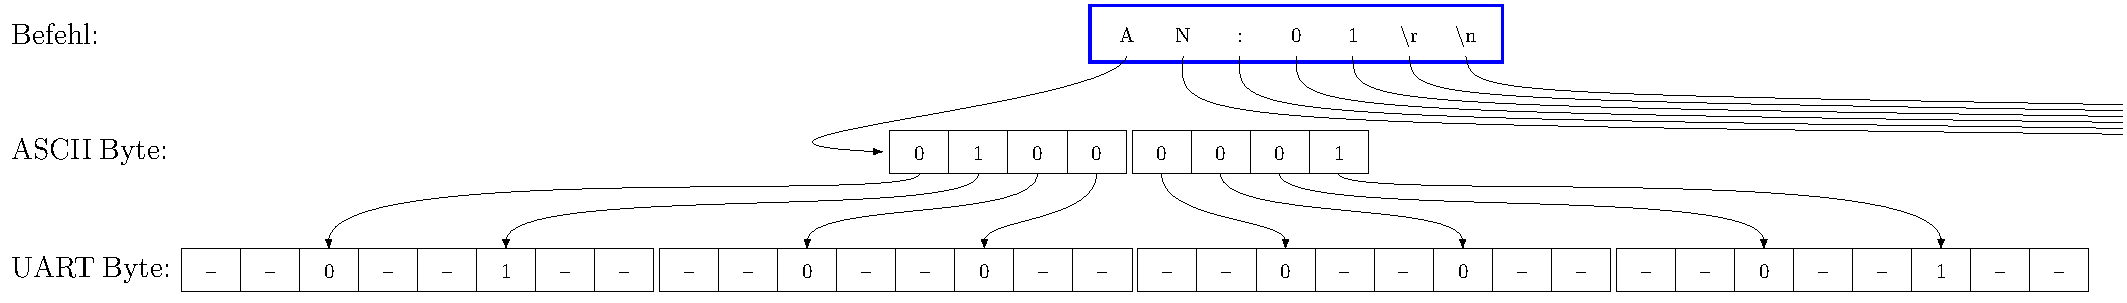
\includegraphics[scale=0.6]{images/UART-Bytes}
    \caption{Umrechnung }
    \label{fig:uart}
  \end{center}
\end{figure}



\section{Libraries und Frameworks}
Diese Arbeit nutzt "`libraries"' und "`frameworks"'.
"`libraries"' sind thematisch gebündelte Funktionen und Routinen. Sie bieten eine \ac{API}, die das eigene Programm ansprechen kann.

"`frameworks"' sind noch mehr und bieten ganze Programmiergerüste und Routinen. Sie rufen wenn nötig selbst vorgesehene Funktionen auf und folgen damit dem Paradigma des "`Inversion of Control"'.

In der aktuellen Version bieten beide nicht nur leicht zugängliche Aufrufe, sondern sind auch sicher und robust in ihrem Gebiet.

\subsection{Serielle Kommunikation}
Bei dem Versuch die Grätedatei direkt anzusprechen kam es zu Problemen, die in Abschnitt~\ref{subsec:kommunikationGeraetedateiLibserialLibrary} erörtert werden. Für die zuverlässige serielle Kommunikation kommt daher eine geeignete Library zum Einsatz.

\subsubsection{libserial}
Das selbst entwickelte C++ Programm nutzt "`liberial"'\footnote{\url{https://github.com/crayzeewulf/libserial}} um sicher und zuverlässig über das Gerätelaufwerk mit dem Arduino (und letztlich dem Kaffeevollautomaten) zu kommunizieren.
Diese Bibliothek bietet eine objektorientierte Schnittstelle für alle \ac{POSIX} Systeme und ist unter Linux über die Paketverwaltung installierbar.

\subsection{Speicher- und Austauschformat}
Sowohl bei der Untersuchung des Speichers, als auch am Ende für das aufbereitete Ergebnis, werden Informationen gesammelt, verglichen und öffentlich zugänglich gemacht.
Als beliebtes und flexibles Speicherformat wird \ac{JSON} verwendet.
Es bietet viele Datenformate und ist unbegrenzt verschachtelbar.
In dieser Arbeit werden hauptsächlich Zeichenketten, Zahlen, Unter-Objekte und -Arrays verwendet.

Darüber hinaus kann es leicht vom C++ Programm, der Webseite, oder auch für viele weitere Projekte genutzt werden.

\subsubsection{libjsoncpp}
Die "`libjsoncpp"'\footnote{\url{https://en.wikibooks.org/wiki/JsonCpp}} bietet dem C++ Programm eine Lese- und Syntaxanalyse-Funktion zum Aufnehmen eines \ac{JSON} Ausdrucks, sowie eine Möglichkeit ein \ac{JSON} Objekt kompakt zusammengefasst oder leserfreundlich aufgefächert in einen Ausgabestrom zu schreiben.
Als Ausgabestrom sind reine \ac{JSON} Dateien nach einer Speicherauszugs Aufnahme oder die Standardausgabe im Gebrauch als API vorstellbar.


\subsection{Webseite}
Eine kleine Webseite soll am Ende die ausgelesenen Werte visuell anschaulich präsentieren.
Die JavaScript-Bibliothek jQuery und das Framework Bootstrap helfen dabei dies zügig und ansprechend umzusetzen.

\subsubsection{Bootstrap}
Bootstrap\footnote{\url{https://getbootstrap.com/}} ist ein von den Twitter Entwicklern begonnenes Projekt um ursprünglich intern die Verwaltungswerkzeuge zu vereinheitlichen.
Daraus ist aber ein ganzes System an Design Elementen geworden, welches heute sehr populär ist.
\ac{HTML}, \ac{CSS} und \ac{JS} werden zusammen eingesetzt und bieten Entwicklern eine Gitteranordnung für eine Mobile- und die Desktop-Ansicht, Inhaltselemente wie Tabellen und Abbildungen oder auch einzelne Komponenten wie Steckkarten, Prozentanzeigen und Knöpfe.

\subsubsection{jQuery}
jQuery\footnote{\url{https://jquery.com/}} ist eine freie \acl{JS}-Bibliothek, die in der "`slim"'-Variante bereits über Bootstrap eingebunden ist.
Um später wirklich mit dem Kaffeevollautomaten interagieren zu können, wird unter anderem \acs{AJAX} aus dem vollständigen jQuery Paket benötigt (auch wenn daraus später ein synchrones JavaScript mit \acs{JSON} wird).

Über das \acs{CDN} eingebundene Packet stehen ab jetzt einfache \aclp{API} zum modifizieren der \acs{HTML} Elemente, ein erweitertes Event-System, sowie \acs{AJAX}-Funktionalitäten bereit.

\subsubsection{Intro.js}
Zu guter Letzt folgt mit Into.js\footnote{\url{https://introjs.com/}} noch eine Schritt-für-Schritt-Anleitung, die dem Seitenbenutzer eine kurze Einführung in den Aufbau und die Bedienung der Webseite geben soll.
